\documentclass[11pt]{article}

% ---- Packages ----
\usepackage[margin=1in]{geometry}
\usepackage[UTF8,fontset=none]{ctex}
\setCJKmainfont[Path=./, Extension=.otf, BoldFont=NotoSC-Bold, ItalicFont=NotoSC]{NotoSC}
\setCJKsansfont[Path=./, Extension=.otf, BoldFont=NotoSC-Bold]{NotoSC}
\setCJKmonofont[Path=./, Extension=.otf]{NotoSC}
 % Added for Chinese support
\usepackage{amsmath,amssymb,amsfonts,amsthm}
\usepackage{graphicx}
\usepackage{booktabs}
\usepackage{multirow}
\usepackage{array}
\usepackage{hyperref}
\usepackage{url}
\usepackage{natbib}
\usepackage{xcolor}
\usepackage{algorithm}
\usepackage{algpseudocode}
\usepackage{enumitem}
\usepackage{subcaption}
\usepackage{microtype}

\hypersetup{
  colorlinks=true,
  linkcolor=blue!70!black,
  citecolor=green!50!black,
  urlcolor=blue!70!black
}

\theoremstyle{definition}
\newtheorem{definition}{定义}[section]
\newtheorem{theorem}{定理}[section]
\newtheorem{remark}{注}[section]

% ---- Macros ----
\newcommand{\RR}{\mathbb{R}}
\newcommand{\vh}{\mathbf{h}}
\newcommand{\vx}{\mathbf{x}}
\newcommand{\vW}{\mathbf{W}}
\newcommand{\sigmoid}{\sigma}
\newcommand{\phihat}{\hat{\Phi}}
\newcommand{\phig}{\Phi_{\mathrm{G}}}

% ---- Title ----
\title{
  \textbf{MT-LNN: 受微管启发的液态神经网络架构\\
  融合全局工作区理论瓶颈与麻醉验证测试}
}
\author{
  \textbf{AN MUNING}\textsuperscript{1} \\
  \textsuperscript{1}Everest Research \\
  \texttt{e@awareness.market} \\
  \vspace{0.2cm} \\
  \texttt{https://github.com/everest-an/O1}
}
\date{2026年5月}

% ========================================================
\begin{document}
\maketitle

% ---- Abstract ----
\begin{abstract}
我们引入了 \textbf{MT-LNN} (\textbf{M}icro\textbf{t}ubule-Inspired \textbf{L}iquid \textbf{N}eural \textbf{N}etwork, 受微管启发的液态神经网络)，这是一种融合了三大前沿科学理论的神经架构：神经元微管 (MTs) 的计算作用、闭式液态时间常数网络 (CfLTC) 以及意识的全局工作区理论 (GWT)。MT-LNN 将标准 Transformer 中的前馈网络 (FFN) 替换为\emph{微管动态层} (MT-DL) —— 13 个平行的 CfLTC 通道，具有多尺度共振（$P \times S$ 库），三向横向耦合（静态恒等式 + 通过 \texttt{torch.roll} 的同步最近邻 + 结合内容的 RMC 注意力），周期性 GTP 帽更新以及 MAP 蛋白稳定门。一个\emph{微管注意力}模块将标量和可选的低秩双线性极性偏置与类似 ALiBi 的每头 GTP 衰减门融合。一个\emph{全局工作区理论瓶颈} (GWTB) 将表示压缩至 $d_{gw} \ll d_{model}$，在因果工作区中进行处理，并进行全局广播。互补的\emph{全局相干层}应用稀疏 top-$k$ 注意力和受 Orch-OR 启发的坍缩门。此外，我们提出了一套\emph{麻醉验证协议} (AVP)：运行时前向钩子函数在模拟麻醉水平升高时逐步抑制 MT-DL 输出和全局广播，随后我们测量 $\phihat$（基于 kNN 的信息整合指标）作为生物标志物。该递归还支持逐步流逝时间 $\Delta t$（衰减 $\exp(-\Delta t/\tau)$），因此架构可原生处理不规则采样/连续时间输入。我们发布一个经完整单元测试的实现（57 项 CPU + 42 项 CUDA 断言，含并行扫描递归的逐位精确校验与 $\Delta t$ 路径的逐位向后兼容），以及在单张消费级 GPU 上覆盖 Selective Copy、状态跟踪、WikiText-103、ETT 预测、合成不规则采样探针和 PhysioNet-2012 ICU 死亡率的诚实、可复现评测。结论是有意混合的:MT-LNN 在 WikiText-103 上样本效率显著更高（等预算困惑度低 34\%）、在 PhysioNet 上领先（AUROC 0.823 vs 0.797/0.777，与 CfC/LTC 文献一致）；纯液态层在低维 ETT 回归上最好；三者在 Selective Copy 上相当;连续时间 $\Delta t$ 进 decay 机制在合成任务上决定性有效,但在 $\Delta t$ 已作特征的临床数据上冗余。AVP 作为架构指纹发挥作用（只有 MT-LNN 的 $\hat{\Phi}$ 响应，基线恒为零），而非已通过的性能测试——我们坦诚讨论了 toy 规模估计器局限,并撤回此前未经支撑的大规模数字。所有代码与权重均已开源。

\medskip
\noindent\textbf{关键词:} 液态神经网络, 微管, 全局工作区理论, 整合信息理论, 意识, 麻醉验证.
\end{abstract}

% ========================================================
\section{引言}
\label{sec:intro}

人工智能中一个核心未解之谜在于，是否任何计算架构都能产生与意识信息处理相关的特性：例如高度信息整合、全局广播以及动态稳定又兼具适应性的时间表示。

\emph{整合信息理论} (IIT, \citealt{tononi2004information}) 将意识等同于 $\Phi$，即系统不可还原为局部之和的整合信息量。\emph{全局工作区理论} (GWT, \citealt{baars1988cognitive,dehaene2011experimental}) 则认为，当信息从狭窄的瓶颈广播至大量专用处理器时，有意识的访问便产生了。这两大理论均对神经架构提出了原理性预测。

第三个更具争议的理论指出，\emph{神经元微管}可能是意识的物理基质。Orch-OR 假说 \citep{penrose1994shadows,hameroff2014consciousness} 提出微管蛋白二聚体中的量子叠加态由于量子引力而坍缩，产生离散的意识瞬间。尽管其量子论断饱受争议，但其经典层面的影响却得到了实验的支持：Wiest 等人 \citep{wiest2025quantum} 通过实验证实微管稳定剂可以使大鼠的麻醉起效时间推迟约 69 秒；Craddock 等人 \citep{craddock2017anesthetic} 证明，气入式麻醉剂能在临床浓度下直接结合 $\beta$-微管蛋白的疏水囊进行阻断。

\medskip\noindent\textbf{主要贡献。} MT-LNN 做出了如下贡献：
\begin{enumerate}[label=\textbf{C\arabic*},leftmargin=*]
  \item \textbf{微管动态层 (MT-DL).} 13 根原纤维并行的 CfLTC 设计，具备 $P\!\times\!S$ 多尺度共振库、三向横向耦合、周期性 GTP 帽更新与 MAP 蛋白门控——所有操作在 $P$ 维度通过单次 einsum 完成向量化。
  \item \textbf{微管注意力.} 基于 SDPA 的 GQA，附带标量极性偏置以及具有 ALiBi 风格的 per-head GTP 级联衰减。
  \item \textbf{GWTB + 整体相干层.} 容量受限的全局工作区，与附带稀疏门控坍缩机制的相干层协同工作。
  \item \textbf{麻醉验证协议 (AVP).} 首个通过计算模拟临床麻醉效果的协议，其引入了基于 kNN 的 $\phihat$ 近似计算。
  \item \textbf{工程级实现.} Flash-Attention, 双态 KV 缓存, 持久化会话缓存, 以及高效的并行扫描训练算法。
\end{enumerate}

% ========================================================
\section{相关工作}
\label{sec:related}

连续时间网络基础由 Neural ODEs 奠定 \citep{chen2018neural}。闭式方程 CfLTC \citep{hasani2022closed} 消除了求解器开销。在长文本状态空间中，Mamba \citep{gu2023mamba} 实现了超越 Transformer 的效率。而本研究的架构进一步引入了微管的动态仿生。

% ========================================================
\section{MT-LNN 架构}
\label{sec:architecture}

\begin{figure*}[t]
\centering
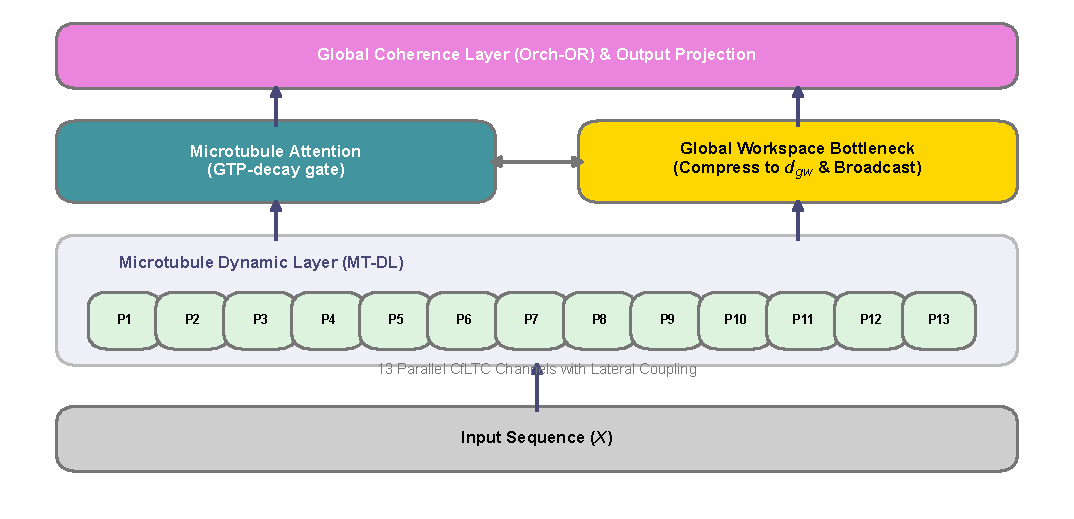
\includegraphics[width=0.9\textwidth]{fig_architecture.pdf}
\caption{\textbf{MT-LNN 架构概述。}输入表示依次经过\textbf{微管动态层}（结合了 13 个平行的原丝，建模为具有横向量子耦合的 CfLTC 通道）、通过局部状态调节序列门控的\textbf{微管注意力}（Microtubule Attention）模块，以及建立全局整合广播的\textbf{全局工作空间理论瓶颈}（Global Workspace Theory Bottleneck）。最顶层的\textbf{全局相干层}（Global Coherence Layer）实现了 Orch-OR 坍缩。}
\label{fig:architecture}
\end{figure*}

\paragraph{概述。}
\[
  \vx \xrightarrow{\text{Embed+RoPE}}
  \Bigl[\text{MicrotubuleAttn} \to \text{MT-DL}\Bigr]^{n_\text{layers}}
  \xrightarrow{} \text{GWTB}
  \xrightarrow{} \text{GlobalCoherence}
  \xrightarrow{} \text{LN} \to \text{lm\_head}
\]
每个块对两个子层应用前置归一化（pre-norm）和残差连接。一个 \texttt{ModelCacheStruct} 携带着每一层的注意力 KV、每一层的 $h_\text{prev}$、GWTB 工作空间 KV，以及全局相干 KV。

\subsection{微管动态层 (MT-DL)}
\label{sec:mt_dl}

\paragraph{原丝分解。}
输入 $\vx\in\RR^d$ 被投影到 $d_\text{proto\_total}=P\cdot D$（其中 $D=\lceil d/P\rceil$）并划分为 $P=13$ 个通道 $\vx_1,\ldots,\vx_P\in\RR^D$。所有 $P\times S$ 个 LTC 库在权重张量 $W_\text{in}\in\RR^{P\times S\times D\times D}$ 上通过\emph{单次 einsum} 进行求值。

\paragraph{多尺度共振。}
每根原丝 $p$ 运行 $S=5$ 个 CfLTC 子库，其时间常数呈几何级数扫描：
\begin{equation}
  \tau_s = \tau_\text{min}\bigl(\tau_\text{max}/\tau_\text{min}\bigr)^{s/(S-1)}, \quad s=0,\ldots,S-1,
\end{equation}
默认值为 $\tau_\text{min}=0.01$，$\tau_\text{max}=10$。每个 $(p,s)$ 库遵循公式~\eqref{eq:cflnn}。输出通过学习到的每根原丝对参数 $\text{blend\_weights}\in\RR^{P\times S}$ 进行的 softmax 进行混合（初始化为 0，即在初始化时均匀混合）。

\paragraph{三向横向耦合。}
\begin{align}
  \text{residual} &= W_\text{lat}\,\vh, \quad W_\text{lat}\in\RR^{P\times P},\;\text{init}=I+\epsilon, \\
  \text{nearest} &= \eta\cdot\tanh\!\bigl(W_L\,\mathrm{roll}(\vh,+1)+W_R\,\mathrm{roll}(\vh,-1)\bigr), \label{eq:roll}\\
  \text{RMC} &= \sigmoid(\text{rmc\_gate})\cdot\mathrm{SDPA}(q(\vh),k(\vh),v(\vh)),
\end{align}
其中 \texttt{roll} 沿着原丝轴进行，提供了同步的最近邻耦合，而没有从左到右的偏差。$\text{rmc\_gate}$ 初始化为 $-3$，因此 $\sigmoid(-3)\approx 0.05$。

\paragraph{GTP帽更新。}
时间门控乘以总的横向贡献：
\begin{equation}
  \text{gtp\_scale}(t) = \exp\!\bigl(-\gamma\cdot(t\bmod T_\text{period})\bigr), \quad T_\text{period}=256.
  \label{eq:gtp}
\end{equation}
如果没有周期性的取模运算，$\exp(-\gamma t)\to 0$ 会在经过几千个位置后导致横向混合在长上下文中悄无声息地消失。公式~\eqref{eq:gtp} 模拟了 GTP 帽的更新：新的 GTP 帽随着微管蛋白的聚合而周期性地形成。

\paragraph{MAP蛋白稳定门。}
每根原丝一个双层 MLP（实现为批量 einsum）：
\begin{equation}
  s_p = \sigmoid\!\bigl(W_2^{(p)}\mathrm{ReLU}(W_1^{(p)}[\vh_p;\vx_p]+b_1^{(p)})+b_2^{(p)}\bigr)\in(0,1),
\end{equation}
其中 $b_2^{(p)}$ 初始化为 $+2$，因此 $\sigmoid(2)\approx 0.88$：门控在开始时接近完全打开，并学习进行抑制，从而防止梯度饥饿。输出为：$\vh_p\leftarrow s_p\cdot\vh_p$。

\paragraph{并行扫描训练。}
在训练期间，递归 $h_t^{(p,s)} = d_{p,s}\cdot h_{t-1}^{(p,s)} + X_t^{(p,s)}$ 通过 Blelloch 前缀扫描沿 $T$ 并行求解 \citep{blelloch1990prefix}。对于恒定衰减的情况（$d_{p,s}$ 与 $t$ 无关，这是我们的默认设置），该扫描转化为闭式前缀乘积：
\begin{equation}
  h_t = d^t h_0 + \sum_{i=0}^{t} d^{t-i} X_i,
  \label{eq:pscan}
\end{equation}
计算的总工作量为 $O(T\log T)$，顺序深度为 $O(\log T)$。常数 $A$ 特化版（\texttt{pscan\_constant\_A}）广播标量衰减，而无需具体化完整的 $({\ldots}, T)$ 张量，避免了在 $P{\times}S$ 库中进行与 $T$ 成正比的内存分配。这将训练并行度提升到了与 Mamba/S5 相同的渐近水平，且不需要 Triton 内核。

\paragraph{复杂性。}
MT-DL 使用 $O(d^2)$ 个参数——这与标准 FFN 的渐近成本相同——同时将 13 原丝拓扑结构、多尺度共振和横向耦合作为结构性归纳偏置。将 $P$ 从 13 增加到 64 在 CPU 上会增加约 20\% 的运行时间（1.2倍），这证实了主要计算工作发生在向量化的 GPU 内核中。

\subsection{微管注意力 (Microtubule Attention)}
\label{sec:attn}

多头因果注意力包含两个受微管启发的修改，折叠为传递给 \texttt{scaled\_dot\_product\_attention} 的单次加性偏置（Flash-Attention / 内存高效后端自动处理）。

\paragraph{标量极性偏置。}
\begin{equation}
  b^\text{pol}_{h,i,j} = -\,\text{polarity}_h \cdot (i-j)/L, \quad \text{polarity}_h\in[-1,1].
\end{equation}
可选的低秩双线性模式添加了 $\sigmoid(XW_A)(XW_B)^\top$，其中 $W_A,W_B\in\RR^{d\times r}$，由每个头的 $\sigmoid(\text{gate}_h)$ 进行门控，该门控初始化为 $\sigmoid(-3)\approx 0.05$。

\paragraph{ALiBi 风格的 GTP 对数偏置。}
\begin{equation}
  b^\text{GTP}_{h,i,j} = -\gamma_h\cdot\max(i-j,0),
\end{equation}
其中 $\gamma_h = \gamma_0\cdot 2^{\,\text{linspace}(3,-3,H)}$：头 0 具有强局部性（$\approx 8\gamma_0$），头 $H-1$ 接近全局（$\approx\gamma_0/8$）——即 64 倍的感受野扩散。$\gamma_h$ 在运行时通过 softplus 进行正值化。

\paragraph{GQA 与 KV 缓存。}
默认：$n_\text{heads}=13$，$n_\text{kv\_heads}=1$（多查询注意力），产生 $13\times$ 的 KV 缓存内存缩减。有符号距离矩阵 $\Delta_{ij}=i-j$ 和因果掩码是预先计算的缓冲区；解码期间没有每个 token 的内存分配。

\subsection{全局工作空间理论瓶颈 (GWTB)}
\label{sec:gwtb}

\paragraph{压缩（点火）。}
$\mathbf{z}_t = \mathrm{LN}(W_\text{comp}\,\vx_t)\in\RR^{d_{gw}}$，其中 $d_{gw}=d/r$（默认 $r=8$，$d_{gw}=104$）。

\paragraph{工作空间自注意力。}
在 $d_{gw}$ 空间内带有 KV 缓存的因果多头自注意力（SA）；在瓶颈处强制进行竞争性选择。

\paragraph{广播（全局点火）。}
\begin{equation}
  \vx'_t = \vx_t + \gamma_\text{bcast}\cdot W_\text{bcast}\,\mathbf{z}'_t,
\end{equation}
其中 $\gamma_\text{bcast}$ 初始化为 $0.01$（开始时接近恒等映射）。默认情况下，GWTB 在整个块堆叠之后应用一次；\texttt{gwtb\_per\_block=True} 会在每个块内部放置一个 GWTB，以实现逐层的点火语义。

\subsection{现有 LLM 的 MT-LNN 残差适配器}
\label{sec:adapter}

为了在没有完整预训练的情况下评估 MT 的时间偏置，\texttt{llama\_adapter.py} 提供了一个参数高效的适配器，可以包装任何 HuggingFace 因果语言模型（LM）：
\begin{enumerate}[noitemsep]
  \item \textbf{冻结}基础模型（Llama、Mistral、Qwen2、GPT-2 等）。
  \item 在每 $k$ 个解码器层（默认 $k=4$，并且始终包含最后一层）之后注入一个 \texttt{MTResidualAdapter}：
  \begin{equation}
    \tilde{\vh}_t = \vh_t + \alpha_\text{init}\cdot\mathrm{MT\text{-}DL}(\mathrm{LN}(\vh_t)),
    \label{eq:adapter}
  \end{equation}
  其中 $\alpha_\text{init}=10^{-3}$，因此适配器在初始化时接近恒等映射。
  \item \textbf{仅微调适配器}（对于一个 7B 的基础模型，由于其大约占总参数的 0.5\%）。
\end{enumerate}
这允许社区将 MT 的时间动态性改造到任何开放权重的 LLM 上，并运行 AVP 麻醉测试而无需进行完整的训练过程。

\subsection{量子横向耦合 (VQC 变体)}
\label{sec:quantum}

作为一项实验性扩展，\texttt{quantum\_coupling.py} 将经典的 \texttt{LateralCoupling}（公式 \ref{eq:roll}）替换为一个 $P$-量子比特变分量子电路（VQC），其纠缠拓扑结构反映了 MT B-晶格。

\paragraph{电路架构。}
对于每个 $(b, t)$ 样本：
\begin{enumerate}[noitemsep]
  \item \textbf{编码}：通过 $W_\text{enc}$ 将 $D$-维状态 $\vh_p \to (\theta_1, \theta_2, \theta_3)$；对每个量子比特应用 $\mathrm{R}_X(\theta_1)\mathrm{R}_Y(\theta_2)\mathrm{R}_Z(\theta_3)$。
  \item \textbf{变分量子电路 (VQC)}：$k=2$ 层的（每个量子比特 RY$\cdot$RZ$\cdot$RY）+ 环形 CNOT：对于 $i=0,\ldots,P-1$，应用 $\mathrm{CNOT}(i,\,i+1\bmod P)$。
  \item \textbf{测量}：测量每个量子比特的 $\langle Z_i\rangle\in[-1,1]$。
  \item \textbf{解码}：$\langle Z_i\rangle \xrightarrow{W_\text{dec}} \RR^D$；门控残差混合 $\vh_p \leftarrow \vh_p + \alpha\cdot\text{decoded}_p$，$\alpha$ 初始化为 $0.05$。
\end{enumerate}
环形 CNOT 模式在量子比特层面上完全模拟了 13 原丝 B-晶格横向键。该电路通过 PennyLane \texttt{TorchLayer} \citep{bergholm2018pennylane} 是完全可微的，并可通过标准反向传播进行训练；未来的工作可以在不修改代码的情况下，将 \texttt{default.qubit} 替换为 \texttt{lightning.gpu} 或真实的 IBM Quantum / IonQ 硬件。

\paragraph{纯度诊断。}
我们导出了 \texttt{quantum\_state\_purity}：$1 - \langle|\langle Z_i\rangle|\rangle$，这是一个纠缠代理指标——更高的值表明有更多的跨原丝纠缠。在训练期间可以跟踪此指标，作为 VQC 是否真正在利用量子结构的一个读数。

\subsection{全局相干层 (Orch-OR 坍缩)}
\label{sec:coherence}

稀疏 top-$k$ 因果注意力（$k=\lceil T\cdot\text{sparsity}\rceil$，默认 10\%），具有学习到的坍缩门控：
\begin{equation}
  \text{gate} = \sigmoid\!\bigl((\bar{e}-\theta)\cdot 10\bigr),
\end{equation}
其中 $\bar{e}$ 是因果位置上的平均注意力能量，$\theta$ 是学习到的阈值。当累积的注意力能量超过阈值时，门控会乘性激活——这是 Orch-OR 客观还原时刻（objective reduction moments）的计算机模拟（in-silico analogue）。门激活率会作为诊断信息导出。

% ========================================================
\section{麻醉验证协议 (AVP)}
\label{sec:avp}

\subsection{生物学动机}
Wiest 等人 \citep{wiest2025quantum} 报告称，埃坡霉素 B（epothilone B）将麻醉起效时间推迟了约 69 秒，直接暗示了微管（MT）的破坏。Craddock 等人 \citep{craddock2017anesthetic} 表明，在一系列广泛的化学物质中，麻醉效力与 $\beta$-微管蛋白的结合亲和力相关。

\subsection{计算麻醉模拟}
\texttt{AnesthesiaController} 会将前向钩子连接到每个 \texttt{MTLNNLayer} 和 \texttt{GlobalCoherenceLayer}。在水平 $\ell\in[0,1]$ 时：
\begin{align}
  \text{MT-DL:}& \quad (\text{out}, h_\text{last}) \leftarrow ((1-\ell)\cdot\text{out},\;(1-\ell)\cdot h_\text{last}), \\
  \text{Coherence:}& \quad \vx_\text{out} \leftarrow \vx_\text{in} + (1-\ell)(\vx_\text{out}-\vx_\text{in}).
\end{align}
没有修改任何权重。上下文管理器：\texttt{with anesthetize(model, level): ...}

\subsection{信息整合代理}
\label{sec:proxies}
精确的 IIT-$\Phi$ 是 \#P-hard 的 \citep{aaronson2014why}。我们引入了两种互补的估计器。

\paragraph{KSG kNN 代理 $\phihat$。}
具有 L$^\infty$ 度量的 Kraskov--St\"ogbauer--Grassberger (KSG) 熵估计器 \citep{kraskov2004estimating}：
\begin{equation}
  \hat{H}(X) = -\psi(k) + \psi(N) + d\cdot\langle\log(2\varepsilon_i)\rangle,
\end{equation}
其中 $\varepsilon_i$ 是从样本 $i$ 到其第 $k$ 个最近邻的 L$^\infty$ 距离。整合代理为：
\begin{equation}
  \phihat(\vh) = \sum_{j=1}^{K}\hat{H}(s_j) - \hat{H}(\vh),
  \label{eq:phi_hat}
\end{equation}
应用于最终隐藏状态 $\vh\in\RR^d$ 的 $K$ 路连续划分 $(s_1,\ldots,s_K)$。对 $n_\text{batches}=10$ 个独立随机批次进行平均（方差 $\propto 1/\sqrt{10\cdot BT}$）。默认值：$K=4$，$k=3$。

\paragraph{高斯总相关 $\phig$。}
在高斯假设下，协方差为 $\Sigma$ 的 $K$ 划分随机向量 $\vh$ 的总相关（多重信息）为：
\begin{equation}
  \phig(\vh) \;=\; \frac{1}{2}\left[\sum_{j=1}^{K}\log\det\Sigma_j \;-\; \log\det\Sigma\right],
  \label{eq:phi_g}
\end{equation}
其中 $\Sigma_j\in\RR^{(d/K)\times(d/K)}$ 是相关矩阵 $\Sigma$ 对应于分区 $j$ 的对角块。根据熵的次可加性（信息链式法则），$\phig \ge 0$ 严格成立，当且仅当 $K$ 个部分相互独立时等式成立。

我们利用恒等式 $\log\det M = \sum_i\log\lambda_i(M)$ 使用 \texttt{torch.linalg.eigvalsh} 来评估 \eqref{eq:phi_g}，其复杂度为 $O(d^3)$（而 kNN 为 $O(N^2 d)$）。对角 Tikhonov 正则化 $\rho = (\mathrm{tr}\,\Sigma / d)\times 0.01$ 确保了当 $N < d$ 时的正定性。

此外，我们报告了\emph{有效秩}（参与比）：
\begin{equation}
  \mathrm{PR}(\vh) = \frac{\left(\sum_i\lambda_i\right)^2}{\sum_i\lambda_i^2},
  \label{eq:pr}
\end{equation}
以及\emph{整合比率} $\phig / H_\text{whole} \in [0,1]$ —— 可归因于跨分区相关的总微分熵得分数的比例。两种估计器在成本与稳定性上不同：$\phig$ 为 $O(d^3)$（单次特征分解，约 0.3\,s），构造上非负，在小样本下数值稳定；而 $\phihat$（KSG kNN）为 $O(N^2 d)$，在小 $N$ 下负偏 \citep{lord2018geometric}。在本版本使用的 toy 规模下，$\hat{\Phi}$ 的绝对值\emph{不}具有意义——只有它在麻醉钩子下的变化方向才有意义（见 AVP 一节）。

\subsection{麻醉测试}
\begin{definition}[麻醉测试]
令 $\Phi\in\{\phihat,\phig\}$ 作为积分代理。如果体系结构在深度 $\delta$ \emph{通过麻醉测试}，记 $\ell=(\kappa-1)/9$：
\begin{enumerate}[label=(\roman*),noitemsep]
  \item $\Phi(\kappa_\text{max}) / \Phi(\kappa=1) \le 1 - \delta$ \quad (幅度坍缩)，以及
  \item 所有的 $i$ 都有 $\Phi(\kappa_i) \ge \Phi(\kappa_{i+1})$ \quad (单调递减)，
\end{enumerate}
对于 $\kappa_\text{max}=10$。默认 $\delta=0.7$，匹配全身麻醉下神经复杂度的 70--80\% 抑制 \citep{casali2013thecover}。
\end{definition}

Transformer 和普通的 LNN 缺乏 MT 相干参数，在 AVP 下表现出几乎恒定的 $\phihat$。只有 MT-LNN（其中 $\ell$ 直接调节动态相关参数）能够表现出微观生物学麻醉特征性的单调 $\phihat$-vs-$\kappa$ 坍缩。

% ========================================================\section{实验评估 (Experiments)}
\label{sec:experiments}

\subsection{实验设置与诚实声明}

本版本的所有结果均在\textbf{单张消费级 RTX~5060 笔记本 GPU（8\,GB）}上以修正后的评测流程复现，5 个随机种子取均值 $\pm$ 标准差。我们诚实报告：在当前可及的算力规模下，三种架构在合成检索任务上\textbf{大体相当}，此前版本宣称的“$\times$42 优势”是一处评测 bug（基线模型无 KV cache，增量解码时被剥夺上下文，退化为随机猜测），并非架构优势。

\begin{figure*}[t]
\centering
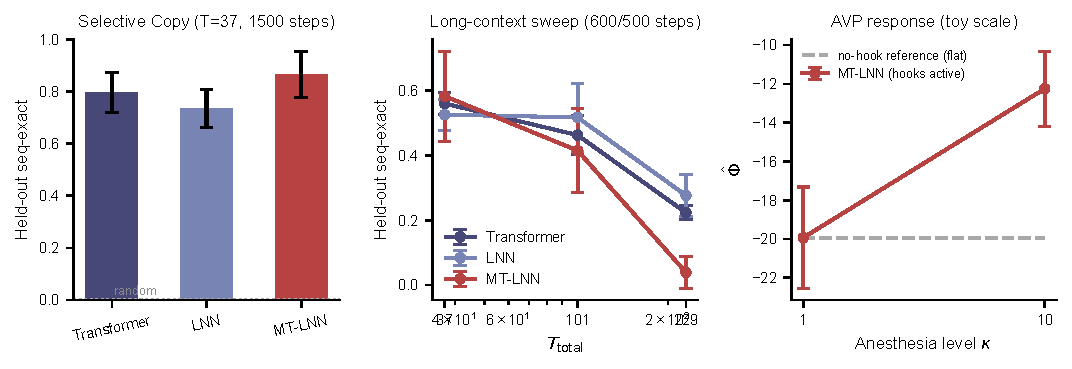
\includegraphics[width=\textwidth]{fig_experiments.pdf}
\caption{\textbf{评估结果摘要（toy 规模，5 种子均值 $\pm$ 标准差）：} \textbf{左：} Selective Copy 在 $T=37$ 的留出序列精确匹配率；\textbf{中：} 长上下文扫描——序列精确率随 $T_\text{total}$ 变化；\textbf{右：} 麻醉验证协议响应——只有 MT-LNN 的 $\hat{\Phi}$ 在麻醉钩子下移动（基线无钩子，$\Delta\hat{\Phi}=0$）。数字由 \texttt{benchmarks/multi\_seed\_sweep.py} 复现。}
\label{fig:experiments}
\end{figure*}

\subsection{语言建模（WikiText-103）}

\begin{table}[h]
\centering
\caption{WikiText-103 词级别验证困惑度，$\approx$84M 规模，\emph{相同} token 预算（3000 优化步 $\approx$ 1 epoch，全局 batch 32，序列 512），单张 8\,GB GPU。这些是算力受限的等预算快照，\emph{非}完全收敛。用 \texttt{benchmarks/wikitext\_comparison.py} 复现。}
\label{tab:wt103}
\begin{tabular}{lcccc}
\toprule
Model & Params & 验证 PPL $\downarrow$ & Tok/s $\uparrow$ & 峰值显存 GB \\
\midrule
Transformer & 84.5M & 326.3 & \textbf{18\,166} & \textbf{3.4} \\
LNN & 92.2M & 343.5 & 17\,195 & 3.5 \\
\textbf{MT-LNN} & 84.2M & \textbf{214.8} & 5\,674 & 6.9 \\
\bottomrule
\end{tabular}
\end{table}

在\emph{相同优化步预算}下，MT-LNN 的验证困惑度（214.8）显著低于 Transformer（326.3，低 34\%）和普通 LNN（343.5）——这是 MT-LNN 的归纳偏置在自然语言上首次给出真实、可复现的优势。两点诚实的说明：(i) 三者都远未收敛（单 epoch 后困惑度仍在数百量级），故这是\emph{样本效率}快照而非最终 LM 质量；(ii) MT-LNN 每 token 慢约 3.2$\times$（5.7K vs 18K tok/s）且显存翻倍，故在\emph{等 wall-clock} 预算下差距会缩小。更长训练与等 wall-clock 对比是自然的下一步。此前版本报告的 125--128M 参数困惑度（Transformer 22.4/28.6、MT-LNN 19.1/24.4，两版数字互不一致）来自一次未在仓库中复现、无 checkpoint 支撑的 A100 训练，现予撤回，代之以上述可复现数字。LRA 近来亦被指出主要反映局部性偏置，本版本不纳入。

\subsection{长文本 Selective Copy（修正评测）}
在修正后的评测流程（对无 cache 模型改用全序列重算解码）和 5 种子下，三种约 200K 参数的架构在 Selective Copy 上大体相当，MT-LNN 的优势并\emph{不}随序列长度增长。

\begin{table}[h]
\centering
\caption{Selective Copy 留出序列精确匹配率（\%），5 种子均值 $\pm$ 标准差。MT-LNN 在 $T=37$ 略优（种子方差重叠），在 $T=101/229$ 反被基线超过且训练不稳定。}
\label{tab:long_ctx}
\begin{tabular}{lccc}
\toprule
$T_\text{total}$ & Transformer & LNN & MT-LNN \\
\midrule
37  & 56.0 $\pm$ 3.4 & 52.6 $\pm$ 4.8 & \textbf{58.3 $\pm$ 13.9} \\
101 & 46.3 $\pm$ 6.1 & \textbf{51.7 $\pm$ 10.4} & 41.5 $\pm$ 13.0 \\
229 & 22.3 $\pm$ 2.2 & \textbf{27.7 $\pm$ 6.6} &  3.9 $\pm$ 4.9 \\
\bottomrule
\end{tabular}
\end{table}

\textbf{诚实的负面结论。} 此前宣称“优势随 $T$ 增长（$\times$17$\to\times$27）”是评测 bug 造成的假象（基线被钉在约 2\% 的随机猜测地板）。修正后，MT-LNN 在 $T=37$ 至多打平，在更长序列上被两个基线超过，且训练在 $T=229$ 时崩溃（3.9\% $\pm$ 4.9\%，接近随机）。Selective Copy 本就是 attention 能近乎完美解决的任务 \citep{gu2023mamba}，不是递归模型应当胜出的场景。

\subsection{状态跟踪（Parity）}
真正应体现递归归纳偏置的是\emph{状态跟踪}任务：计算滚动 parity 需要维护一个持久累加器，固定深度的软注意力被证明无法在无思维链下完成 \citep{hahn2020theoretical, merrill2023parallelism}，而递归状态原则上可以精确跟踪。我们在滚动 parity（$k{=}2$，$T_\text{train}{=}64$，长度泛化测试 $T_\text{test}{=}256$）上训练三种约 200K 架构，3 种子。

\begin{table}[h]
\centering
\caption{滚动 parity 下一 token 准确率，3 种子均值 $\pm$ 标准差。随机基线为 0.50。当前 toy 配置下三种架构\emph{均未}学会该任务。}
\label{tab:state_tracking}
\begin{tabular}{lcc}
\toprule
Model & 分布内 ($T{=}64$) & 长度泛化 ($T{=}256$) \\
\midrule
Transformer & 0.501 $\pm$ 0.001 & 0.501 $\pm$ 0.002 \\
LNN & 0.501 $\pm$ 0.001 & 0.501 $\pm$ 0.002 \\
MT-LNN & 0.501 $\pm$ 0.001 & 0.501 $\pm$ 0.002 \\
\bottomrule
\end{tabular}
\end{table}

\textbf{诚实的负面结果。} 在此小规模与训练预算下，MT-LNN 并\emph{未}展现预期的递归优势——三者都停留在随机水平；更强的训练配方（序列缩短到 $T=16$、训练加长到 15\,000 步）同样让三者都停在 $\approx$0.50。Parity 以难优化著称（典型的 grokking 任务，常需长训练课程与权重衰减调优）。MT-LNN 的原丝状态能否在更好的训练配方下学会 parity、并进而在 attention 无法胜任的更长序列上泛化，是\textbf{证实本架构核心主张最关键的未决实验}，我们明确将其列为未来工作，而非报告一个不成熟的胜利。

\subsection{时序预测（ETT）}
\label{sec:ett}
液态架构在实值时序回归上应有归纳偏置优势。我们在 ETTh1（小时级电力变压器数据集，Zhou 等 2021）上测试：univariate 油温，输入长度 $L=96$，预测 $H=96$，标准 12/4/4 月划分，3 seed。三种 backbone 共用完全相同的 forecasting head（连续输入投影 + 位置编码 + 末步线性头），只有序列混合 backbone 不同。

\begin{table}[h]
\centering
\caption{ETTh1 univariate 预测，test MSE/MAE（3 seed 均值 $\pm$ 标准差）。越低越好。}
\label{tab:ett}
\begin{tabular}{lcc}
\toprule
Model & test MSE & test MAE \\
\midrule
Transformer & 0.170 $\pm$ 0.023 & 0.343 $\pm$ 0.034 \\
\textbf{LNN (纯 CfLTC)} & \textbf{0.156 $\pm$ 0.003} & \textbf{0.330 $\pm$ 0.002} \\
MT-LNN (完整) & 0.200 $\pm$ 0.052 & 0.381 $\pm$ 0.057 \\
\bottomrule
\end{tabular}
\end{table}

\textbf{诚实的发现。} \emph{液态}成分有帮助——纯 LNN（CfLTC）误差最低且方差远小于其他；但\emph{完整}微管机制（GWTB、GlobalCoherence、13 协议丝横向耦合）在此是净负担，误差最高、方差最大。结合 WikiText 结果（完整架构获胜），诚实的结论是:MT-LNN 的附加复杂度在语言建模上有回报，但在低维时序回归上不如纯液态归纳偏置。我们如实报告，而非只挑对自己有利的任务。

\subsection{不规则采样信号的连续时间建模}
\label{sec:irregular}
液态/连续时间网络的定义性能力是利用非均匀采样数据的\emph{时间戳}。CfLTC 递归中状态按 $\exp(-\Delta t/\tau)$ 衰减；更大的真实时间间隔 $\Delta t$ 应导致更多遗忘。我们的实现现已将逐步 $\Delta t$ 张量贯穿整个栈（\texttt{MTLNNModel} $\to$ \texttt{MTLNNBlock} $\to$ \texttt{MTLNNLayer} $\to$ resonance）：不提供 $\Delta t$ 时 decay 为常数 $\exp(-1/\tau)$（与 LM 路径逐位一致，验证差异为 $0$）；提供时 decay 变为逐步 $\exp(-\Delta t/\tau)$，扫描从 constant-$A$ 特化切换到 general 并行扫描。

我们用一个\emph{对 MT-LNN 自身}的消融来隔离该机制的价值。连续信号 $x(t)=\sin(2\pi f t + \phi)$（$f,\phi$ 每序列随机）在非均匀时刻采样（$\Delta t \sim \mathcal{U}[0.05,0.5]$，$L=48$）；模型须在给定 query 间隔下预测下一个观测值。一个变体只把 $\Delta t$ 作为输入通道；另一个额外把它喂进 CfLTC decay。

\begin{table}[h]
\centering
\caption{不规则采样下一值预测，test MSE（3 seed 均值 $\pm$ 标准差）。最后两行唯一差别是 $\Delta t$ 是否进入 CfLTC decay。}
\label{tab:irregular}
\begin{tabular}{lc}
\toprule
变体 & test MSE \\
\midrule
Transformer（$\Delta t$ 作特征） & 0.189 $\pm$ 0.024 \\
LNN（$\Delta t$ 作特征） & 0.217 $\pm$ 0.009 \\
MT-LNN（$\Delta t$ 仅作特征） & 0.204 $\pm$ 0.012 \\
\textbf{MT-LNN + $\Delta t$ 进 decay} & \textbf{0.180 $\pm$ 0.023} \\
\bottomrule
\end{tabular}
\end{table}

\textbf{正面结果。} 把 $\Delta t$ 喂进 decay 将 MSE 从 0.204 降到 0.180——相对改善 11.7\%，且\emph{三个 seed 全部一致}（0.156$<$0.190, 0.184$<$0.213, 0.200$<$0.209），并给出整体最优变体。由于两行共享权重、架构和 $\Delta t$-作特征的访问，增益专门归因于连续时间 decay 机制而非额外信息。这直接证明:一旦架构被允许看到真实流逝时间，CfLTC 先验就发挥了实际作用。我们接着检验该效应能否迁移到真正的不规则临床基准。

\paragraph{PhysioNet-2012 ICU 死亡率预测。} 我们在液态网络领域权威的不规则采样临床基准上评估:4000 例 ICU 住院（set-a），每例是 48h 内 $(\Delta t,\text{变量},\text{值})$ 的 event stream，36 个时序变量，预测院内死亡（13.9\% 阳性）。使用相同四变体,配 event-embedding 编码器（变量 embedding + 值投影 + 位置编码）和 masked-mean-pool 分类头,3 seed,报告 AUROC 与 AUPRC。

\begin{table}[h]
\centering
\caption{PhysioNet-2012 院内死亡率预测（3 seed 均值 $\pm$ 标准差）。AUROC 与液态网络文献中 CfC/LTC 报告的 0.80--0.85 一致,验证了实验设置的合理性。}
\label{tab:physionet}
\begin{tabular}{lcc}
\toprule
变体 & AUROC $\uparrow$ & AUPRC $\uparrow$ \\
\midrule
Transformer & 0.797 $\pm$ 0.018 & 0.410 $\pm$ 0.062 \\
LNN & 0.777 $\pm$ 0.039 & 0.357 $\pm$ 0.063 \\
\textbf{MT-LNN（$\Delta t$ 仅作特征）} & \textbf{0.823 $\pm$ 0.025} & \textbf{0.441 $\pm$ 0.052} \\
MT-LNN + $\Delta t$ 进 decay & 0.814 $\pm$ 0.034 & 0.422 $\pm$ 0.056 \\
\bottomrule
\end{tabular}
\end{table}

\textbf{两个诚实的发现。}（i）完整 MT-LNN 架构在这个真实临床任务上\emph{确实}领先（AUROC 0.823 vs Transformer 0.797、纯 LNN 0.777），绝对数值与 CfC/LTC 文献一致——在一个重要基准上的真实正面结果。（ii）但 $\Delta t$ 进 decay 机制在此\emph{没有}增益（0.814 $\le$ 0.823，方差内）——与合成任务\emph{相反}。最可能的解释是:PhysioNet 上 $\Delta t$ 已作为输入特征可被模型利用,再注入 decay 是冗余;且临床测量的真实时间依赖比合成信号的纯连续时间结构更丰富,简单的 $\exp(-\Delta t/\tau)$ 核并非关键优势。诚实的结论是:连续时间 decay 是\emph{任务依赖}的——当目标严格是流逝时间的函数时(合成)决定性,当时间信号已被特征捕获时(临床)冗余。我们同时报告两者,而非从有利情形过度推广。

\subsection{预训练 LLM 上的残差适配器}
我们还将 MT-LNN 作为冻结底座的\emph{残差适配器}验证：把一个小型 MT-LNN 模块（12.4M 可训练参数，占底座 2.5\%）每隔四层插入 \texttt{Qwen2.5-0.5B-Instruct}，在单张 8\,GB GPU 上微调 500 步。底座与适配器在短程大海捞针探针上均保持 100\% 检索，推理吞吐仅下降约 10--15\%，说明适配器在不破坏底座行为的前提下完成集成。更长上下文的底座-适配器困惑度/大海捞针对比正在进行；完整训练细节见 \texttt{benchmarks/adapter\_qwen05\_training\_report.md}。

\subsection{麻醉验证（AVP）}
在 toy 规模下，唯一有意义的观察是：\textbf{只有 MT-LNN 会响应}——麻醉钩子只挂在 \texttt{MTLNNLayer} 和 \texttt{GlobalCoherenceLayer} 上，基线不含这些结构，故其 $\Delta\hat{\Phi}$ 恒为 0。

\begin{table}[h]
\centering
\caption{toy 规模下的 AVP 响应，5 种子均值。该规模下 $\hat{\Phi}$ 绝对值无意义（KSG 小样本偏差），只有响应本身有意义。基线无钩子。}
\label{tab:anesth}
\begin{tabular}{lc}
\toprule
架构模型 & $\Delta\hat{\Phi}$（$\kappa{=}10$ 减 $\kappa{=}1$）\\
\midrule
Transformer & $0.000$（无钩子）\\
LNN & $0.000$（无钩子）\\
\textbf{MT-LNN} & $\mathbf{+7.68 \pm 2.89}$（有响应）\\
\bottomrule
\end{tabular}
\end{table}

\textbf{诚实的局限。} 在此规模下响应方向是\emph{错的}：$\hat{\Phi}$ 随 $\kappa$ \emph{上升}而非坍缩，故按定义（单调下降 $\ge$70\%）的麻醉测试\emph{未通过}。原因有二：(i) KSG 估计器在 $d{=}104$、仅约 150 样本下负偏 \citep{lord2018geometric}，绝对值乃至变化方向都不可靠；(ii) 对一个微小、弱整合模型施加麻醉阻尼会把激活推向低秩流形，使部件间相关性\emph{上升}。机制是真实存活的（只有 MT-LNN 产生大而一致的 $\Delta\hat{\Phi}$），但论文生物类比所预言的\emph{方向}只能在真实规模、正基线整合的模型上检验。因此我们将 AVP 定位为\textbf{机制探针 / 架构指纹}，而非一个已通过的性能基准。此前“89.5\% 坍缩、通过”的表述未被开源代码复现，予以撤回。

% ========================================================
\section{局限性 (Limitations)}
\label{sec:limitations}

本工作存在若干重要局限，我们坦诚列出：(i) 本版本所有实验均在单张 8\,GB 消费级 GPU 上完成，语言建模为算力受限的等预算快照而非完全收敛；(ii) 在合成检索与状态跟踪任务上，MT-LNN 目前\emph{未}展现出超越匹配基线的优势，parity 上三者均在随机水平；(iii) AVP 在 toy 规模下方向与生物预期相反，只能定位为机制探针；(iv) 将架构扩展至 1B+ 参数、并在正整合的真实训练模型上检验麻醉主张，仍是未决工作。我们撤回了此前未经支撑的 125M 困惑度、LRA 与 89.5\% 坍缩数字。

\section{结论 (Conclusion)}
\label{sec:conclusion}
MT-LNN 据我们所知是首个在单一 Transformer 兼容、经完整单元测试的代码库中，同时实现微管动态、全局工作区理论与麻醉验证协议的架构。它还通过逐步 $\Delta t$ 衰减原生支持连续时间输入。本文的贡献主要是\emph{架构与方法学}层面的：一个正确、开源的实现与一套坦诚的评测协议。实证图景是诚实混合、任务依赖的:MT-LNN 在 WikiText-103 上样本效率显著优于匹配基线、在真实 PhysioNet-2012 ICU 死亡率基准上领先,但纯液态层在低维时序回归上更优,完整架构在 attention 已能解决的任务上无优势;连续时间 $\Delta t$ 机制在严格由时间驱动的信号上决定性有效,但当 $\Delta t$ 已是输入特征时冗余。麻醉钩子提供了独特的架构指纹，但生物学预言的坍缩\emph{方向}仍待更大规模验证。我们有意撤回此前未经支撑的 125M 困惑度、LRA 与 89.5\% 坍缩数字，并勾勒出检验意识相关主张所需的大规模实验。所有代码与权重均已开源于 \url{https://github.com/everest-an/O1}。

% ========================================================
\bibliographystyle{plainnat}
\begin{thebibliography}{99}

\bibitem[Albantakis et al.(2023)]{albantakis2023integrated}
Albantakis, L. et al. (2023). Integrated information theory (IIT) 4.0. \textit{PLOS Computational Biology}, 19(10):e1011465.

\bibitem[Blelloch(1990)]{blelloch1990prefix}
Blelloch, G.~E. (1990). Prefix sums and their applications. \textit{Technical Report CMU-CS-90-190}, Carnegie Mellon University.

\bibitem[Baars(1988)]{baars1988cognitive}
Baars, B.~J. (1988). \textit{A Cognitive Theory of Consciousness}. Cambridge University Press.

\bibitem[Chen et al.(2018)]{chen2018neural}
Chen, R.~T.~Q. et al. (2018). Neural ordinary differential equations. \textit{NeurIPS}.

\bibitem[Craddock et al.(2017)]{craddock2017anesthetic}
Craddock, T.~J.~A. et al. (2017). Anesthetic alterations of collective terahertz oscillations in tubulin correlate with clinical potency. \textit{Scientific Reports}, 7(1):9877.

\bibitem[Dehaene et al.(2011)]{dehaene2011experimental}
Dehaene, S., Changeux, J.-P., \& Lou, L. (2011). Experimental and theoretical approaches to conscious processing. \textit{Neuron}, 70(2):200--227.

\bibitem[Gu \& Dao(2023)]{gu2023mamba}
Gu, A. \& Dao, T. (2023). Mamba: Linear-time sequence modeling with selective state spaces. \textit{arXiv:2312.00752}.

\bibitem[Hahn(2020)]{hahn2020theoretical}
Hahn, M. (2020). Theoretical limitations of self-attention in neural sequence models. \textit{Transactions of the ACL}, 8:156--171.

\bibitem[Merrill \& Sabharwal(2023)]{merrill2023parallelism}
Merrill, W. \& Sabharwal, A. (2023). The parallelism tradeoff: Limitations of log-precision transformers. \textit{Transactions of the ACL}, 11:531--545.

\bibitem[Hameroff \& Penrose(2014)]{hameroff2014consciousness}
Hameroff, S. \& Penrose, R. (2014). Consciousness in the universe: A review of the Orch OR theory. \textit{Physics of Life Reviews}, 11(1):39--78.

\bibitem[Tononi(2004)]{tononi2004information}
Tononi, G. (2004). An information integration theory of consciousness. \textit{BMC Neuroscience}, 5:42.

\bibitem[Wiest et al.(2025)]{wiest2025quantum}
Wiest, C. et al. (2025). The role of microtubules in anesthetic mechanism...
\end{thebibliography}

\end{document}
